\documentclass[ngerman, a4, 12pt, listof=totoc]{scrreprt}
\usepackage[a4paper,left=3cm,right=3cm,top=2.5cm,bottom=3.5cm]{geometry}
\usepackage{amsmath}
\usepackage{siunitx}
\usepackage{sidecap}
\usepackage{gensymb}
\usepackage{babel}
\usepackage{xcolor}
\usepackage{graphicx}
\usepackage{lipsum}
\usepackage{listings}
\usepackage{color}
\usepackage{tabularx}
\usepackage{wrapfig}
\usepackage[pdfborder={0 0 0}]{hyperref}
\usepackage[backend=biber,style=alphabetic,sorting=ynt]{biblatex}
\usepackage[autostyle]{csquotes}
\renewcommand{\labelenumi}{\alph{enumi})}
\addbibresource{literatur.bib}

% Not useful with Lua Latex
% \usepackage[utf8]{inputenc}

% Frage: wie man Code inserted

% Mann kann parindent nutzen, um das Einrücken zu verhindern.
% \parindent0pt


\renewcommand\lstlistingname{Quelltext} % Change language of section name
\lstset{ % General setup for the package
    language=Python,
    basicstyle=\small\sffamily,
    numbers=left,
    numberstyle=\small,
    frame=tb,
    tabsize=4,
    columns=fixed,
    showstringspaces=false,
    showtabs=false,
    keepspaces,
    commentstyle=\color{red},
    keywordstyle=\color{blue}
}


\titlehead{\begin{center} 
\includegraphics[width=3cm]{assets/icon.png} \end{center}}
\title{\LaTeX \, Linux}
\subtitle{Das beste Betriebssystem}
\publishers{Mik Müller}

\author{Linus Torvalds}
\date{\today}

\begin{document}
\maketitle

% Man benutzt ein*, damit es nicht im Inhaltsverzeichnis auftaucht  
% Geht auch mit \section \chapter \subsection

\begin{abstract}
    \section*{Abstract}
    \subsection*{Lorem Ipsum}
    \lipsum[1-5]
\end{abstract}

\tableofcontents

\chapter{Einleitung}
\section{Was ist Linux}

Als Linux oder GNU/Linux (siehe GNU/Linux-Namensstreit) bezeichnet man in der Regel freie, unixähnliche Mehrbenutzer-Betriebssysteme, die auf dem Linux-Kernel und wesentlich auf GNU-Software basieren. Die weite, auch kommerzielle Verbreitung wurde ab 1992 durch die Lizenzierung des Linux-Kernels unter der freien Lizenz GPL ermöglicht. Einer der Initiatoren von Linux war der finnische Programmierer Linus Torvalds. Er nimmt bis heute eine koordinierende Rolle bei der Weiterentwicklung des Linux-Kernels ein und wird auch als Benevolent Dictator for Life (deutsch wohlwollender Diktator auf Lebenszeit) bezeichnet.

Das modular aufgebaute Betriebssystem wird von Softwareentwicklern auf der ganzen Welt weiterentwickelt, die an den verschiedenen Projekten mitarbeiten. An der Entwicklung sind Unternehmen, Non-Profit-Organisationen und viele Freiwillige beteiligt. Beim Gebrauch auf Computern kommen meist sogenannte Linux-Distributionen zum Einsatz. Eine Distribution fasst den Linux-Kernel mit verschiedener Software zu einem Betriebssystem zusammen, das für die Endnutzung geeignet ist. Dabei passen viele Distributoren und versierte Benutzer den Kernel an ihre eigenen Zwecke an.

Linux wird vielfältig und umfassend eingesetzt, beispielsweise auf Arbeitsplatzrechnern, Servern, Mobiltelefonen, Routern, Notebooks, Embedded Systems, Multimedia-Endgeräten und Supercomputern. Dabei wird Linux unterschiedlich häufig genutzt: So ist Linux im Server-Markt wie auch im mobilen Bereich eine feste Größe, während es auf dem Desktop und Laptops eine noch geringe, aber wachsende Rolle spielt. Im März 2021 war es in Deutschland auf 2,19 \% der Systeme installiert.

Linux wird von zahlreichen Nutzern verwendet, darunter private Nutzer, Regierungen, Organisationen und Unternehmen.

\chapter{GNU / LINUX}
\section{Stallman's Interjection}

I'd just like to interject for a moment.  What you're referring to as Linux,
is in fact, GNU/Linux, or as I've recently taken to calling it, GNU plus Linux.
Linux is not an operating system unto itself, but rather another free component
of a fully functioning GNU system made useful by the GNU corelibs, shell
utilities and vital system components comprising a full OS as defined by POSIX.

Many computer users run a modified version of the GNU system every day,
without realizing it.  Through a peculiar turn of events, the version of GNU
which is widely used today is often called "Linux", and many of its users are
not aware that it is basically the GNU system, developed by the GNU Project.

There really is a Linux, and these people are using it, but it is just a
part of the system they use.  Linux is the kernel: the program in the system
that allocates the machine's resources to the other programs that you run.
The kernel is an essential part of an operating system, but useless by itself;
it can only function in the context of a complete operating system.  Linux is
normally used in combination with the GNU operating system: the whole system
is basically GNU with Linux added, or GNU/Linux.  All the so-called "Linux"
distributions are really distributions of GNU/Linux.
\chapter{\LaTeX \, Tips}
\section{Grundlagen der Textformatierung}
\subsection{Textarten}

\textbf{Fettgedruckter Text}\\
\emph{Schräger Text}\\
\vspace{1cm}
\underline{Unterstrichen}\\
{\large groß} \\
{\Large größer} \\
{\huge noch Größer} \\
{\Huge noch noch Größer} \\



\subsection{Umbrüche}
Forcierter Zeilenumbruch
\begin{verbatim}
    \\
\end{verbatim}
Forcierter Seitenumbruch
\begin{verbatim}
    \newpage
\end{verbatim}

\subsection{Platzhalter und Abstände}
lorem ipsum \, dolor simet amet\\
lorem ipsum \quad dolor simet amet\\
lorem ipsum \hspace{1cm} dolor simet amet\\
lorem ipsum \vspace{1cm}\\
dolor simet amet\\
lorem ipsum \hfill dolor simet amet\\

\newpage

\section{Listen}
\subsection{Ungeordnet}
Liste 1
\begin{itemize}
    % \itemsep-0.1cm
    \item[-] Item 1
    \item[*] Item 2
    \item[$\rightarrow$] Item 3
    \item[$\triangle$] Item 4
    \item[$\Rightarrow$] Item 5
    \item[$x$] Item 6
\end{itemize}
Liste 2
\begin{itemize}
    \item Normales Item
\end{itemize}
Liste 3
\subsection{Numeriert}
\begin{enumerate}
    \item Item
    \item Item
    \item Item
    \item Item
\end{enumerate}

\section{Programmcode}
\begin{lstlisting}
    print("Hello World!")
    for i in range(31415):
        print("In Loop")
\end{lstlisting}
\chapter{Tabellen}
\section{Normale Tabellen}

\begin{figure}
    \caption{Tabelle}
    \label{Kleine Test Tabelle}
    % Label
    % \label{tab:tabular_table}
    \begin{tabular}{|l|c|r|}
        \hline
        \textbf{Spalte 1}                  & \textbf{Spalte 2} & \textbf{Spalte 3} \\
        \hline
        Inhalt 1                           & Inhalt 2          & Inhalt 3          \\
        \multicolumn{2}{|c|}{Zwei Spalten} & InhaltX                               \\
        \hline
    \end{tabular}
\end{figure}


\section{Größere Tabelle}

\begin{tabular}{|l|c|r|p{5cm}|@{ Spalte 5 }|}
    \hline
    left                             & center                      & right        & Mit fester Breite von 5 cm und Zeilenumbruch            \\
    \cline{1-3}
    Spalte 1                         & Spalte 2                    & Spalte 3     & In Spalte 5 \newline steht immer das gleiche            \\
    \hline
    \multicolumn{3}{|c|}{nicht viel} & aber so sind viele Tabellen                                                                          \\
    \cline{4-4}
    Noch                             & eine                        & Zeile        & ohne viel Inhalt -- aber der stand nicht im Vordergrund \\
    \hline
    Eine                             & leere                       & Zeile        & das geht auch                                           \\
                                     &                             &              &                                                         \\
    Sogar                            & zweimal                     &              &                                                         \\
    \hline
                                     &                             &              &                                                         \\
                                     &                             &              &                                                         \\
    Nur                              & die                         & automatische & Spalte ist ein bisschen anders                          \\
    \hline
    Und                              & nochmal                     & mit          & vline \vline auch \vline es komisch \vline aussieht     \\
    \hline
\end{tabular}

\newpage

\section{Tabellen ausrichten}

\lipsum[1-2]

\begin{table}[h]
    \caption{Eine erweiterte tabularx tabelle}

    % \label{tab:tabularx_table}
    \begin{tabularx}{\textwidth}{|X|X|X|}
        \hline
        \textbf{Spalte1}  & \textbf{Spalte2}  & \textbf{Spalte3}  \\
        \hline
        Inhalt Inhalt 1 1 & Inhalt Inhalt 1 2 & Inhalt Inhalt 1 3 \\
        Inhalt Inhalt 2 1 & Inhalt Inhalt 2 2 & Inhalt Inhalt 2 3 \\
        Inhalt Inhalt 3 1 & Inhalt Inhalt 3 2 & Inhalt Inhalt 3 3 \\
        \hline
    \end{tabularx}
\end{table}

\lipsum[1-2]

\lipsum[1-2]

\begin{figure}[h]
    \centering
    \label{tux}
    
\includegraphics[height=2cm]{assets/icon.png}
    \caption{Das Linux Maskottchen}
\end{figure}

\lipsum[1-2]

\ldots wie in Abbildung \ref{tux} gezeigt, \ldots
Hier ist jemand: \cite{einstein} \cite{knuth-fa}
% Zeigt alles im Verzeichnis an
\nocite{*}

\color{blue}
\href{https://mik-mueller.de}{Meine Website}
\color{black}

\chapter{Formeln}
\section{Inline}
Hier ist die Formel $f_{(x)}=m \cdot x + b$ für eine Lineare Funktion
\section{Block}
$$f_{(x)}=ax^3+bx^2+cx$$
Oder
\begin{equation}
    f(x) = m \cdot x + b
    \label{Lineare Funktion}
\end{equation}

\section{Labels}
\begin{equation}
    \label{eq:einstein}
    E = mc^2
\end{equation}

Oder um eine \hyperref[eq:einstein]{Formel} referenzieren zu können.

\section{Formel Array}

\begin{eqnarray}
    E &=& mc^2 \qquad \qquad \text{sinnvolle Beschreibung.} \\
    \Leftrightarrow c^2 &=& \frac{E}{m} \\
    c &=& \sqrt{\frac{E}{m}}
\end{eqnarray}

Formeln \footnote{Macht Mathe Zeug} sind toll.


Es ist 5 $\degree$ Celsius.

\section{Rechnungen}
\begin{align*}
     &                 & E   & = mc^2               &  & |\, :m      \\
     & \Leftrightarrow & c^2 & = \frac{E}{m}        &  & |\, \sqrt{} \\
     & \Leftrightarrow & c   & = \sqrt{\frac{E}{m}}                  \\
\end{align*}

\begin{align*}
     & \Leftrightarrow & f(x)=mx+b &  & | \cdot 4
\end{align*}

\chapter{Minipages}

Hier sind  \hyperref[fig:kabel]{Kabel} und \hyperref[fig:server]{Server} zusehen.


\begin{figure}[h]
    \begin{minipage}{.42\linewidth}
        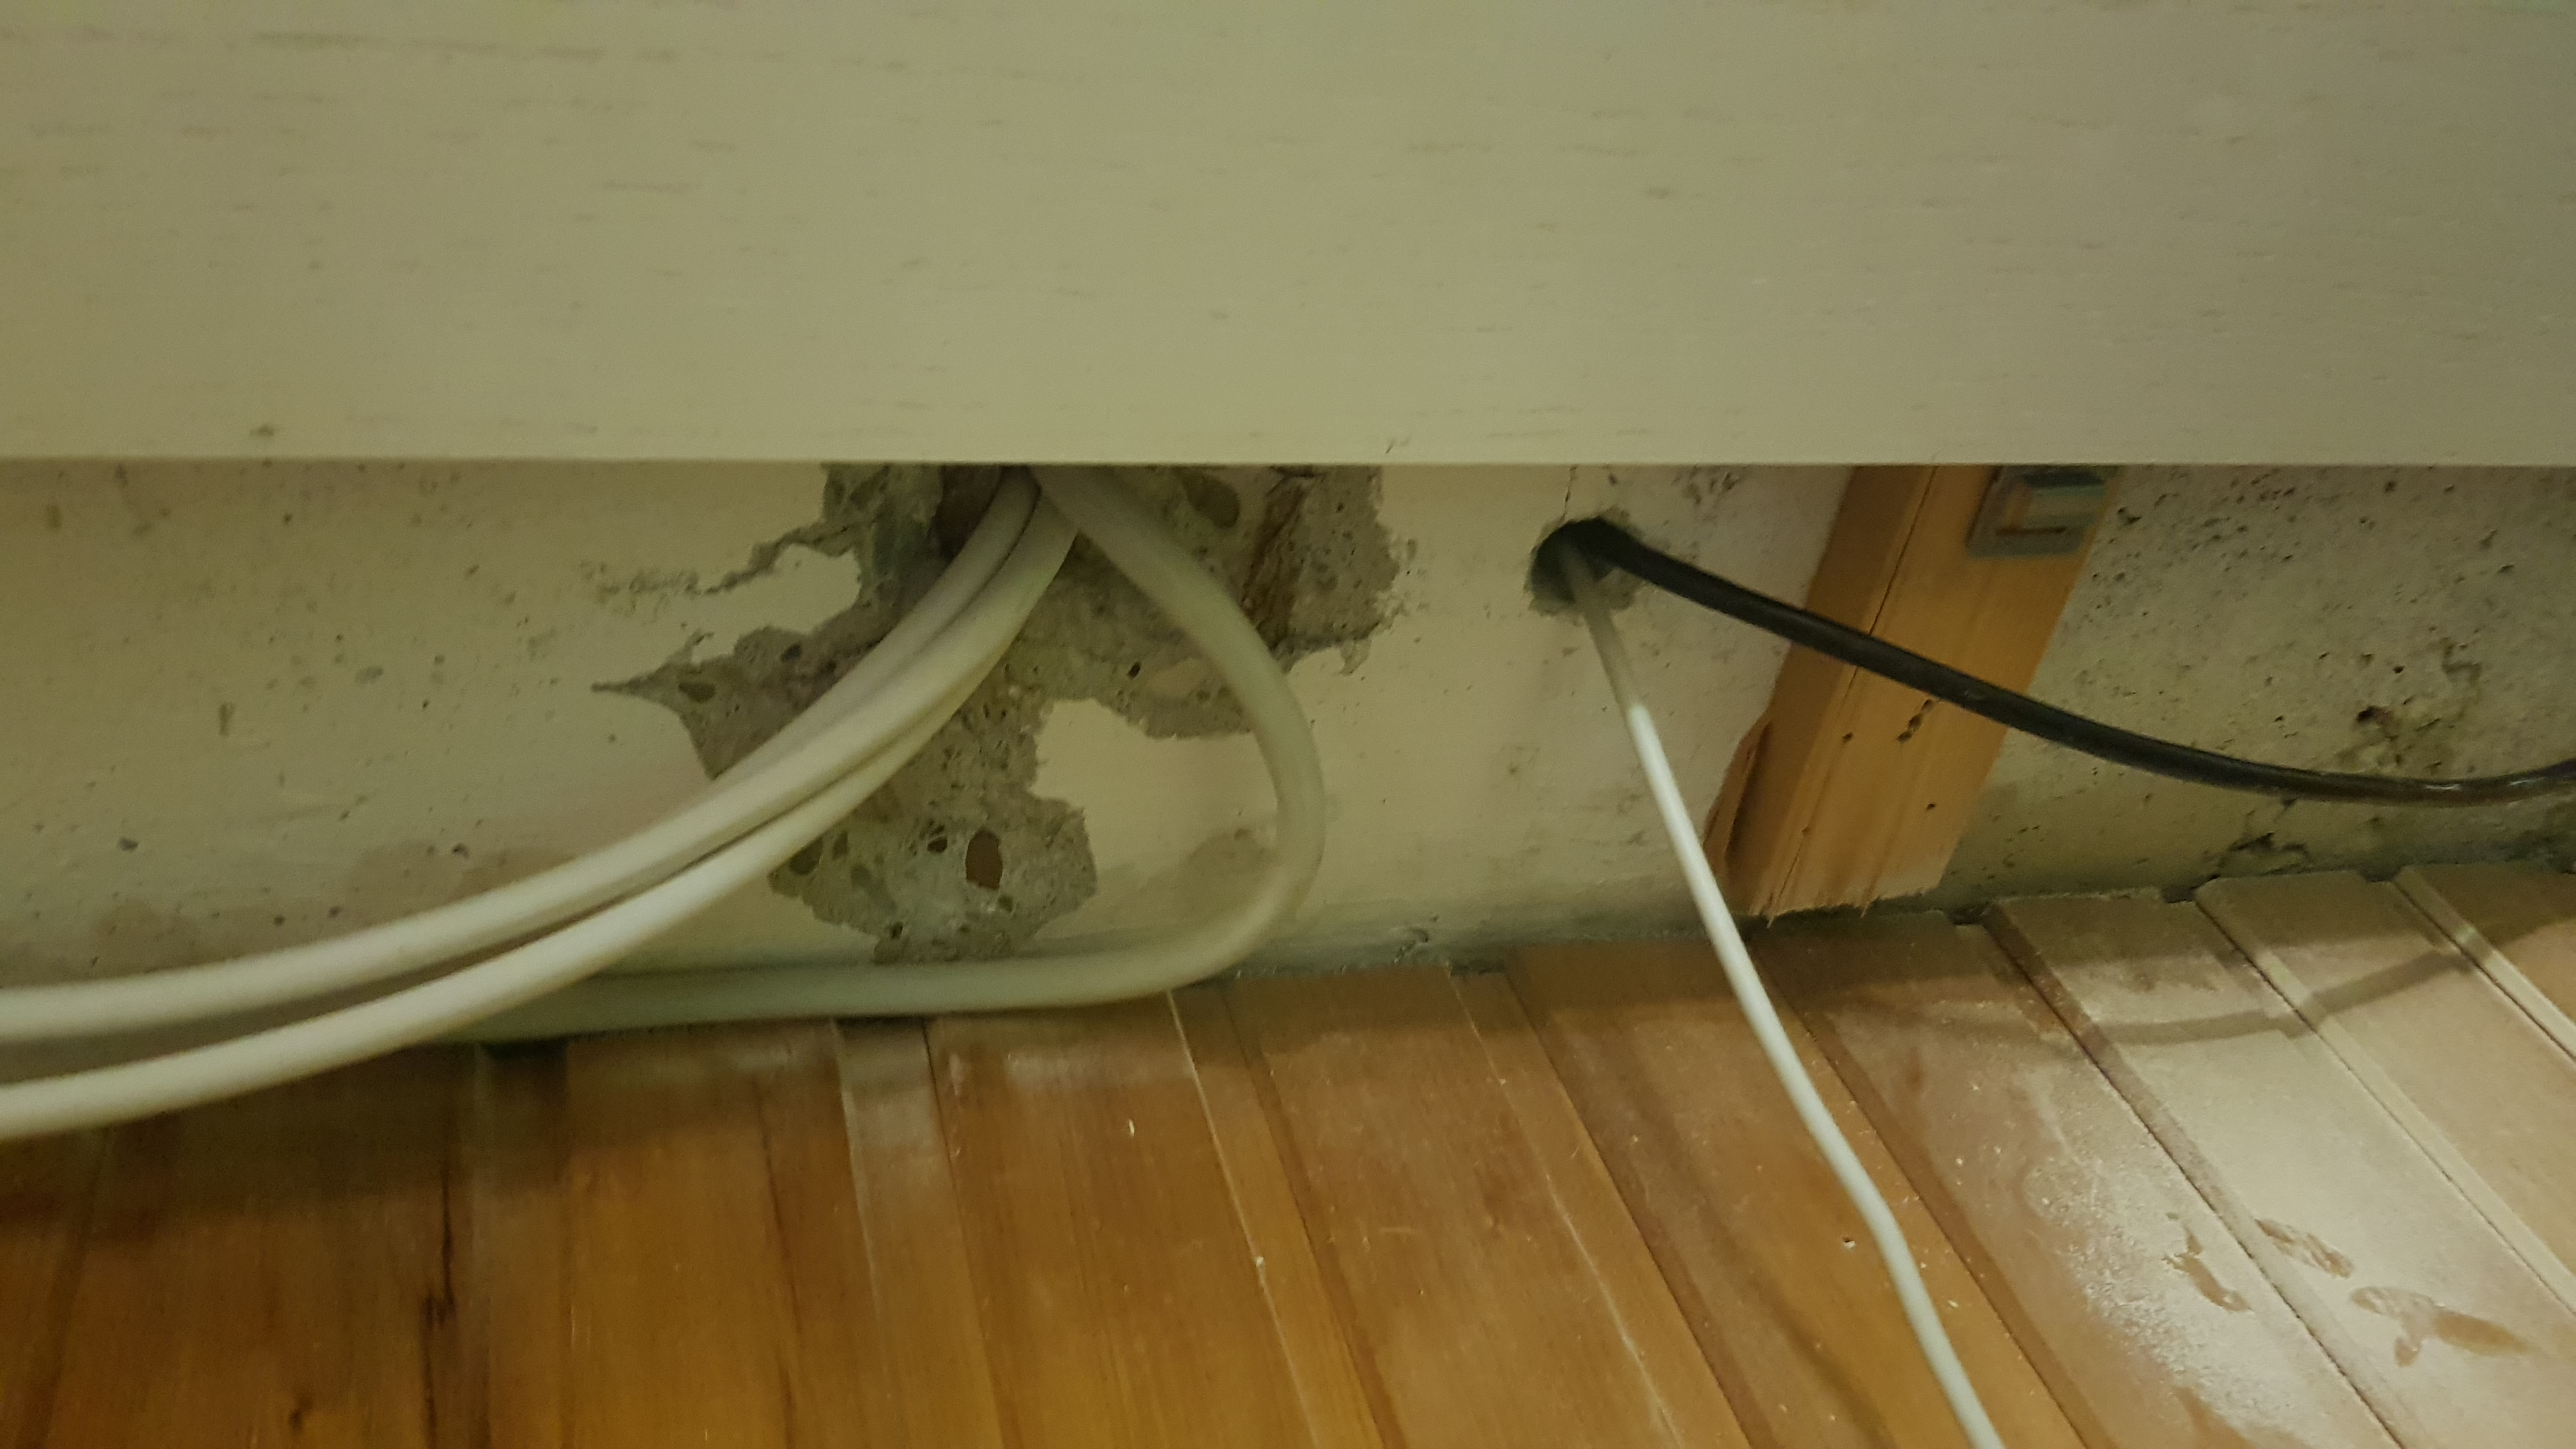
\includegraphics[width=\linewidth]{assets/1.jpg}
        \caption{Kabel}
        \label{fig:kabel}
    \end{minipage}
    \hfill
    \begin{minipage}{.42\linewidth}
        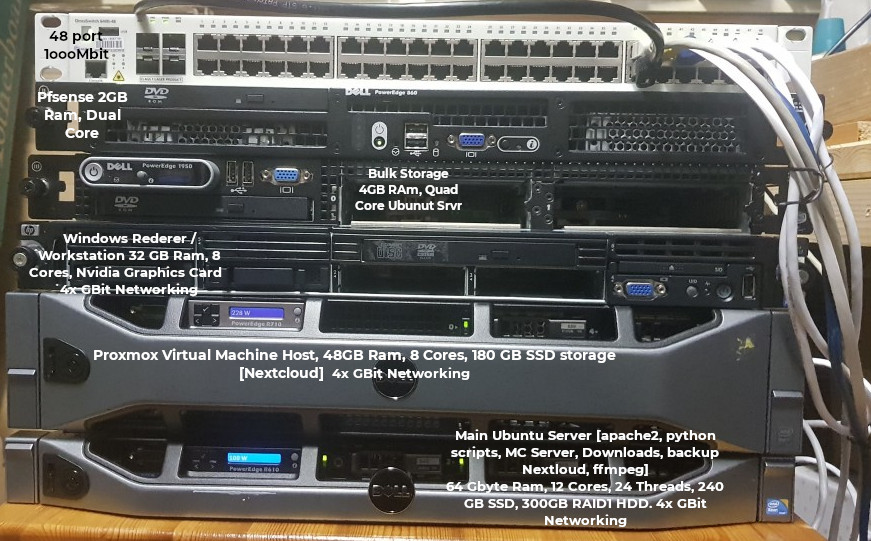
\includegraphics[width=\linewidth]{assets/2.jpg}
        \caption{Server}
        \label{fig:server}
    \end{minipage}
    \centering
    \fcolorbox{red}{gray} {
        \begin{minipage}{.42\linewidth}
            
\includegraphics[width=\linewidth]{assets/icon.png}
            \caption{Tux}
            \label{fig:tux}
            % TODO mach das
        \end{minipage}
    }
\end{figure}

\chapter{Farben}
\color{blue}
\lipsum[1-2]
\color{black}

\textcolor{red}{Roter Text} Text armer Text

\chapter{Side Captions}

\lipsum[1-2]
\begin{figure}[h]
    \caption{This is a caption}
    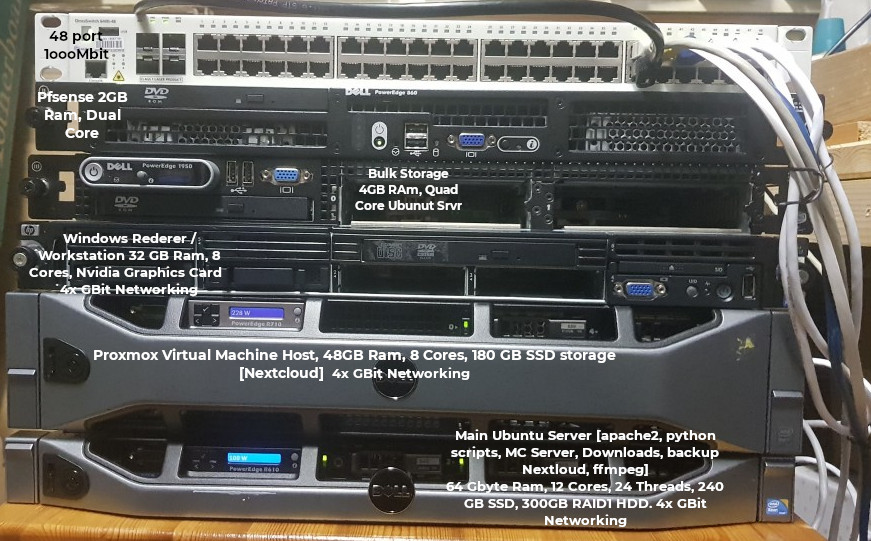
\includegraphics[width=4cm]{assets/2.jpg}
\end{figure}
\lipsum[1-2]


\lipsum[1-2]
\begin{wrapfigure}{r}[0cm]{2cm}
    \raggedleft
    \caption{\label{TestGrafik}}
    
\includegraphics[width=2cm]{assets/icon.png}
\end{wrapfigure}
\lipsum[1-2]


% \begin{SCfigure}
%     \caption{This is a caption}
%     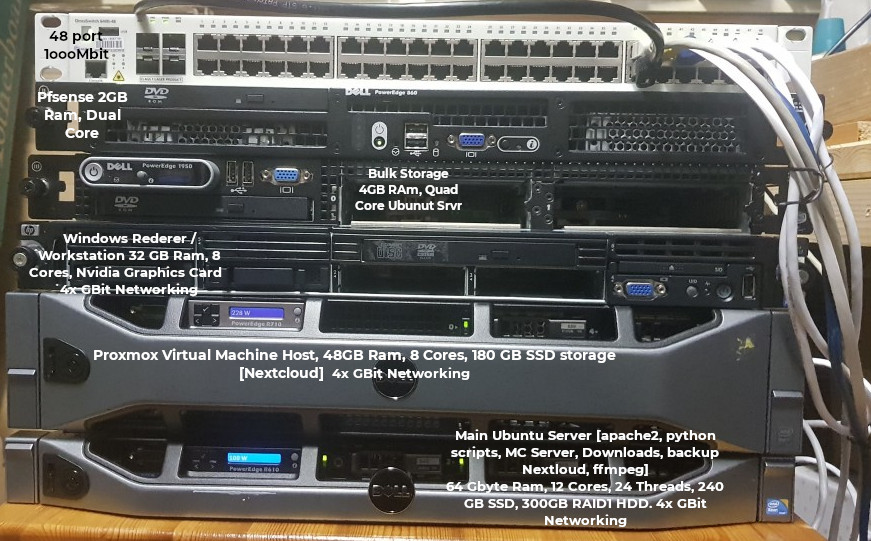
\includegraphics[width=4cm]{assets/2.jpg}
% \end{SCfigure}

$E = mc^2$ \cite{einstein}

\listoffigures
\listoftables
\printbibliography[heading=bibintoc,title={Literaturverzeichnis}]
\end{document}
